\documentclass[a4paper,conference]{IEEEtran}
% This is stripped down to basically the ieee bare_conf.tex header
\usepackage{amssymb,amsmath}
% use upquote if available, for straight quotes in verbatim environments
\IfFileExists{upquote.sty}{\usepackage{upquote}}{}
% use microtype if available
\IfFileExists{microtype.sty}{%
\usepackage{microtype}
\UseMicrotypeSet[protrusion]{basicmath} % disable protrusion for tt fonts
}{}
\usepackage{hyperref}
\PassOptionsToPackage{usenames,dvipsnames}{color} % color is loaded by hyperref
\hypersetup{unicode=true,
            pdftitle={Data Mining- Practice 5},
            pdfborder={0 0 0},
            breaklinks=true}
\urlstyle{same}  % don't use monospace font for urls
% -- biblio. set natbib: true in pandoc for silly hacks around pandoc \cite{} vs \citep{}
\usepackage{cite}
\bibliographystyle{IEEEtran}
\let\citep\cite
% if you want the [2, 3] vs IEEE [2], [3]
\renewcommand{\citepunct}{,\penalty\citepunctpenalty\ }
\usepackage{color}
\usepackage{fancyvrb}
\newcommand{\VerbBar}{|}
\newcommand{\VERB}{\Verb[commandchars=\\\{\}]}
\DefineVerbatimEnvironment{Highlighting}{Verbatim}{commandchars=\\\{\}}
% Add ',fontsize=\small' for more characters per line
\usepackage{framed}
\definecolor{shadecolor}{RGB}{248,248,248}
\newenvironment{Shaded}{\begin{snugshade}}{\end{snugshade}}
\newcommand{\AlertTok}[1]{\textcolor[rgb]{0.94,0.16,0.16}{#1}}
\newcommand{\AnnotationTok}[1]{\textcolor[rgb]{0.56,0.35,0.01}{\textbf{\textit{#1}}}}
\newcommand{\AttributeTok}[1]{\textcolor[rgb]{0.13,0.29,0.53}{#1}}
\newcommand{\BaseNTok}[1]{\textcolor[rgb]{0.00,0.00,0.81}{#1}}
\newcommand{\BuiltInTok}[1]{#1}
\newcommand{\CharTok}[1]{\textcolor[rgb]{0.31,0.60,0.02}{#1}}
\newcommand{\CommentTok}[1]{\textcolor[rgb]{0.56,0.35,0.01}{\textit{#1}}}
\newcommand{\CommentVarTok}[1]{\textcolor[rgb]{0.56,0.35,0.01}{\textbf{\textit{#1}}}}
\newcommand{\ConstantTok}[1]{\textcolor[rgb]{0.56,0.35,0.01}{#1}}
\newcommand{\ControlFlowTok}[1]{\textcolor[rgb]{0.13,0.29,0.53}{\textbf{#1}}}
\newcommand{\DataTypeTok}[1]{\textcolor[rgb]{0.13,0.29,0.53}{#1}}
\newcommand{\DecValTok}[1]{\textcolor[rgb]{0.00,0.00,0.81}{#1}}
\newcommand{\DocumentationTok}[1]{\textcolor[rgb]{0.56,0.35,0.01}{\textbf{\textit{#1}}}}
\newcommand{\ErrorTok}[1]{\textcolor[rgb]{0.64,0.00,0.00}{\textbf{#1}}}
\newcommand{\ExtensionTok}[1]{#1}
\newcommand{\FloatTok}[1]{\textcolor[rgb]{0.00,0.00,0.81}{#1}}
\newcommand{\FunctionTok}[1]{\textcolor[rgb]{0.13,0.29,0.53}{\textbf{#1}}}
\newcommand{\ImportTok}[1]{#1}
\newcommand{\InformationTok}[1]{\textcolor[rgb]{0.56,0.35,0.01}{\textbf{\textit{#1}}}}
\newcommand{\KeywordTok}[1]{\textcolor[rgb]{0.13,0.29,0.53}{\textbf{#1}}}
\newcommand{\NormalTok}[1]{#1}
\newcommand{\OperatorTok}[1]{\textcolor[rgb]{0.81,0.36,0.00}{\textbf{#1}}}
\newcommand{\OtherTok}[1]{\textcolor[rgb]{0.56,0.35,0.01}{#1}}
\newcommand{\PreprocessorTok}[1]{\textcolor[rgb]{0.56,0.35,0.01}{\textit{#1}}}
\newcommand{\RegionMarkerTok}[1]{#1}
\newcommand{\SpecialCharTok}[1]{\textcolor[rgb]{0.81,0.36,0.00}{\textbf{#1}}}
\newcommand{\SpecialStringTok}[1]{\textcolor[rgb]{0.31,0.60,0.02}{#1}}
\newcommand{\StringTok}[1]{\textcolor[rgb]{0.31,0.60,0.02}{#1}}
\newcommand{\VariableTok}[1]{\textcolor[rgb]{0.00,0.00,0.00}{#1}}
\newcommand{\VerbatimStringTok}[1]{\textcolor[rgb]{0.31,0.60,0.02}{#1}}
\newcommand{\WarningTok}[1]{\textcolor[rgb]{0.56,0.35,0.01}{\textbf{\textit{#1}}}}
\usepackage{graphicx,grffile}
\makeatletter
\def\maxwidth{\ifdim\Gin@nat@width>\linewidth\linewidth\else\Gin@nat@width\fi}
\def\maxheight{\ifdim\Gin@nat@height>\textheight\textheight\else\Gin@nat@height\fi}
\makeatother
% Scale images if necessary, so that they will not overflow the page
% margins by default, and it is still possible to overwrite the defaults
% using explicit options in \includegraphics[width, height, ...]{}
\setkeys{Gin}{width=\maxwidth,height=\maxheight,keepaspectratio}

\title{Data Mining- Practice 5}
% for over three affiliations, or if they all won't fit within the width
% of the page, use this alternative format. Cannot use \and or alignment is wrong
\author{\IEEEauthorblockN{%
  Rajesh Kalakoti\IEEEauthorrefmark{4}%
  , Sven Nomm\IEEEauthorrefmark{1}%
}
\IEEEauthorblockA{\IEEEauthorrefmark{1}
      Taltech, Estonia, 12616}
\IEEEauthorblockA{\IEEEauthorrefmark{4}
      Email:
\href{mailto:rajesh.kalakoti@outlook.com}{\nolinkurl{rajesh.kalakoti@outlook.com}}}
}





\date{2023-10-05 14:08:30 +0300}
\setlength{\parindent}{0pt}
\setlength{\parskip}{6pt plus 2pt minus 1pt}
\let\tightlist\relax % silly pandoc thing

% --- user includes
% Put your preamble here. Example.
% subfigures
\usepackage{subfig}
% dots in filenames
\usepackage{graphicx, grffile}
% bold math
\usepackage{bm}
% colours
\usepackage[usenames,dvipsnames]{xcolor}
% suppress month in bibliography
%\AtEveryBibitem{\clearfield{month}}
%\AtEveryCitekey{\clearfield{month}}

% texdef -t latex -f {cmdname} to see if cmd is already defined

% Letters in fancy font (expectation, integers, reals, normal dist)
\newcommand{\E}[1]{\operatorname{\mathbb{E}}{\left[#1\right]}}
\newcommand{\Z}{\mathbb{Z}}
\newcommand{\R}{\mathbb{R}}
\newcommand{\N}{\mathcal{N}}

\begin{document}
\maketitle
\begin{abstract}
As part of our ongoing exploration into this dynamic field, todays's
lecture delves into the intricacies of classification techniques.
Focusing on the versatile R programming language, this session will
unravel the implementation of fundamental algorithms such as Naive
Bayes, Decision Trees, Fisher Score, Gini Index, Entropy.
\end{abstract}

\hypertarget{sec:introduction}{%
\section{Introduction}\label{sec:introduction}}

Classification is a fundamental task in machine learning and data mining
where the goal is to assign a label or category to an input based on its
features. In other words, classification algorithms learn from labeled
training data, allowing them to make predictions or decisions about new,
unseen data. It is widely used in various fields such as email
filtering, speech recognition, image recognition, and sentiment
analysis. you can some articles from medium
\citep{Classifi72:online, Introtot39:online, Lecture045:online}.

\begin{figure}
\centering
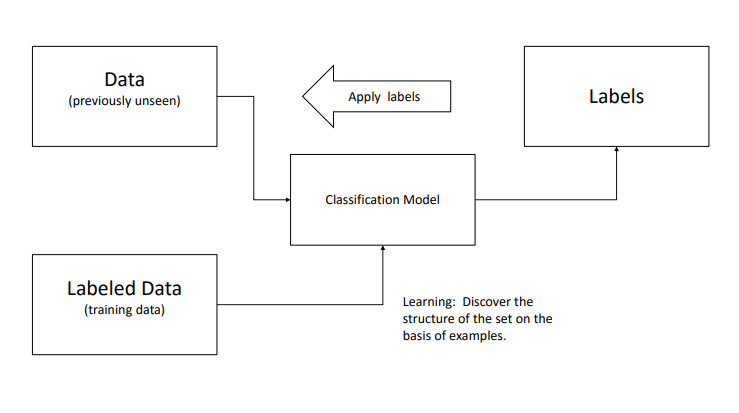
\includegraphics{/home/rajeshkalakoti/Documents/data_mining_with_R/RMarkDown/week5/figure/intro.png}
\caption{Classfication}
\end{figure}

\hypertarget{sec:feature-selection}{%
\section{Feature selection}\label{sec:feature-selection}}

In a dataset with \textbf{n} instances (data points) and \textbf{m}
features (variables), represented as a matrix \textbf{X} of size
\textbf{n × m}, where \(X_{ij}\) represents the value of feature
\textbf{j} for instance \textbf{i}, and \textbf{y} is the corresponding
vector of size \textbf{n} representing the target variable or class
labels.

The objective of \textbf{feature selection} is to find a subset
\(S \subseteq \{1, 2, \ldots, m\}\) of features that maximizes (or
minimizes) an objective function \(J(S)\) representing the performance
of the model. Feature selection aims to optimize the model's performance
by identifying a subset of relevant features, thereby enhancing the
model's accuracy, interpretability, and computational efficiency.

\begin{itemize}
\tightlist
\item
  Filter Methods: A subset of features is evaluated with the use of a
  class-sensitive discriminative criterion.
\item
  Wrapper Methods: Wrapper models evaluate subsets of features using a
  specific machine learning algorithm.
\item
  Embedded Methods: Embedded models integrate feature selection into the
  model training process.
\end{itemize}

\hypertarget{sec:filter-methods}{%
\subsection{Filter Methods}\label{sec:filter-methods}}

\hypertarget{sec:gini-index}{%
\subsubsection{Gini Index}\label{sec:gini-index}}

It measures Measures the discriminative power of a particular feature.
it is used for categorical variables, but it can be generalized to
numeric attributes by the process of discretization. Let
\(v_1, . . . , v_r\) are the possible values of the particular
categorical. Let \(p_j\) denotes the fraction of the data points
containing attribute value \(v_i\) belonging to the class
\(j \in {1, . . . , k}\) to the data points containing attribute value
\(v_i\) then Gini index defined as follows:

\begin{equation}\protect\hypertarget{eq:giniindex}{}{ G(v_i) = 1 - \sum_{j=1}^{k} p_j^2 }\end{equation}

A value of \(1 - \frac{1}{k}\) indicates that the different classes are
distributed evenly for a particular attribute value. Lower value of Gini
Index imply Greater discrimination.

\begin{Shaded}
\begin{Highlighting}[]
\CommentTok{\#\textquotesingle{} gini index}
\CommentTok{\#\textquotesingle{}}
\CommentTok{\#\textquotesingle{} @param probabilities}
\CommentTok{\#\textquotesingle{} Gini index, a measure of impurity }
\CommentTok{\#\textquotesingle{} or inequality, }
\CommentTok{\#\textquotesingle{} for a set of probabilities.}
\CommentTok{\#\textquotesingle{}\textbackslash{}deqn\{G(v\_i) = 1 {-} \textbackslash{}sum\_\{j=1\}\^{}\{k\} p\_j\^{}2\}.}
\CommentTok{\#\textquotesingle{}}
\CommentTok{\#\textquotesingle{} @return}
\CommentTok{\#\textquotesingle{} @export}
\CommentTok{\#\textquotesingle{}}
\CommentTok{\#\textquotesingle{} @examples}
\NormalTok{gini\_score }\OtherTok{\textless{}{-}} \ControlFlowTok{function}\NormalTok{(probabilities) \{}
\NormalTok{  gini\_index }\OtherTok{\textless{}{-}} \DecValTok{1} \SpecialCharTok{{-}} \FunctionTok{sum}\NormalTok{(probabilities}\SpecialCharTok{\^{}}\DecValTok{2}\NormalTok{)}
  \FunctionTok{return}\NormalTok{(gini\_index)}
\NormalTok{\}}

\CommentTok{\# Example probabilities }
\NormalTok{probabilities }\OtherTok{\textless{}{-}} \FunctionTok{c}\NormalTok{(}\FloatTok{0.2}\NormalTok{, }\FloatTok{0.3}\NormalTok{, }\FloatTok{0.5}\NormalTok{)}

\NormalTok{gini\_value }\OtherTok{=} \FunctionTok{gini\_score}\NormalTok{(probabilities)}
\CommentTok{\# Print the result}
\FunctionTok{print}\NormalTok{(gini\_value)}
\end{Highlighting}
\end{Shaded}

\begin{verbatim}
## [1] 0.62
\end{verbatim}

\hypertarget{sec:entropy}{%
\subsubsection{Entropy}\label{sec:entropy}}

The class-based entropy measure is related to notions of information
gain resulting from fixing a specific attribute value. The class- base
entropy is defied as follows:
\begin{equation}\protect\hypertarget{eq:entropy}{}{ E(v_i) = - \sum_{j=1}^{k} p_ilog_2(p_j) }\end{equation}
takes its values in \([0,log_2(k)]\), whereas greater values indicate
greater mixing.

By analogy with Gini index one may define overall Entropy as

\[ E = \sum_{i=1}^{r} \frac{n_iE(v_i)}{n} \] low entropy shall always be
preferred over high entropy

\begin{Shaded}
\begin{Highlighting}[]
\NormalTok{entropy }\OtherTok{\textless{}{-}} \ControlFlowTok{function}\NormalTok{(probs) \{}
  \CommentTok{\# Make sure the probabilities sum up to 1}
  \ControlFlowTok{if}\NormalTok{ (}\FunctionTok{abs}\NormalTok{(}\FunctionTok{sum}\NormalTok{(probs) }\SpecialCharTok{{-}} \DecValTok{1}\NormalTok{) }\SpecialCharTok{\textgreater{}} \FloatTok{1e{-}10}\NormalTok{) \{}
    \FunctionTok{stop}\NormalTok{(}\StringTok{"Probabilities must sum up to 1."}\NormalTok{)}
\NormalTok{  \}}

\NormalTok{  probs }\OtherTok{\textless{}{-}}\NormalTok{ probs[probs }\SpecialCharTok{\textgreater{}} \DecValTok{0}\NormalTok{]}
\NormalTok{  entropy\_value }\OtherTok{\textless{}{-}} \SpecialCharTok{{-}}\FunctionTok{sum}\NormalTok{(probs}\SpecialCharTok{*}\FunctionTok{log2}\NormalTok{(probs))}

  \FunctionTok{return}\NormalTok{(entropy\_value)}
\NormalTok{\}}

\NormalTok{probabilities1 }\OtherTok{\textless{}{-}} \FunctionTok{c}\NormalTok{(}\FloatTok{0.5}\NormalTok{, }\FloatTok{0.5}\NormalTok{) }
\NormalTok{probabilities2 }\OtherTok{\textless{}{-}} \FunctionTok{c}\NormalTok{(}\FloatTok{0.2}\NormalTok{, }\FloatTok{0.8}\NormalTok{)}

\CommentTok{\# Calculate entropy}
\NormalTok{entropy\_value1 }\OtherTok{\textless{}{-}} \FunctionTok{entropy}\NormalTok{(probabilities1)}
\NormalTok{entropy\_value2 }\OtherTok{\textless{}{-}} \FunctionTok{entropy}\NormalTok{(probabilities2)}

\CommentTok{\# Print the results}
\FunctionTok{print}\NormalTok{(}\FunctionTok{paste}\NormalTok{(}\StringTok{"Entropy:"}\NormalTok{, entropy\_value1))}
\end{Highlighting}
\end{Shaded}

\begin{verbatim}
## [1] "Entropy: 1"
\end{verbatim}

\hypertarget{sec:fisher-score.}{%
\subsubsection{Fisher Score.}\label{sec:fisher-score.}}

The Fisher score is naturally designed for numeric attributes to measure
the ratio of the average interclass separation to the average intraclass
separation. The larger the Fisher score, the greater the discriminatory
power of the attribute. Let \(\mu_j\) and \(\sigma_j\) denote the mean
and the standard deviation of the of the data points belonging to the
class \(j\), for a particular feature. And let \(p_j\) be the fraction
of the points belonging to the class \(j\). Finally let \(\mu\) define
the mean of the entire data set. The Fisher index is defined as follows:

\begin{equation}\protect\hypertarget{eq:fisherscore}{}{
F_s = \frac{\sum_{j=1}^{K} p_j(\mu_{j}^{i}-\mu^i)^2}{\sum_{j=1}^{K}p_j (\sigma_{j}^i)^{2}}
}\end{equation}

The attributes with the largest value of the Fisher score may be
selected for use with the classification algorithm.

\begin{Shaded}
\begin{Highlighting}[]
\NormalTok{fisher\_score }\OtherTok{\textless{}{-}} \ControlFlowTok{function}\NormalTok{(data, labels) \{}
  \FunctionTok{cat}\NormalTok{(}\FunctionTok{rep}\NormalTok{(}\StringTok{\textquotesingle{}==\textquotesingle{}}\NormalTok{, }\DecValTok{2}\NormalTok{), }\StringTok{\textquotesingle{}}\SpecialCharTok{\textbackslash{}n}\StringTok{\textquotesingle{}}\NormalTok{)}

\NormalTok{  data\_length }\OtherTok{\textless{}{-}} \FunctionTok{nrow}\NormalTok{(data)}
\NormalTok{  list\_of\_classes }\OtherTok{\textless{}{-}} \FunctionTok{unique}\NormalTok{(labels)}
\NormalTok{  number\_of\_classes }\OtherTok{\textless{}{-}} \FunctionTok{length}\NormalTok{(list\_of\_classes)}
  \FunctionTok{cat}\NormalTok{(}\FunctionTok{paste}\NormalTok{(}\StringTok{"Data contains:"}\NormalTok{, number\_of\_classes, }\StringTok{"classes.}\SpecialCharTok{\textbackslash{}n}\StringTok{"}\NormalTok{))}

\NormalTok{  fishers\_score\_frame }\OtherTok{\textless{}{-}} \FunctionTok{data.frame}\NormalTok{(}\FunctionTok{matrix}\NormalTok{(}\ConstantTok{NA}\NormalTok{, }\AttributeTok{nrow =} \DecValTok{1}\NormalTok{, }\AttributeTok{ncol =} \FunctionTok{ncol}\NormalTok{(data)))}
  \FunctionTok{colnames}\NormalTok{(fishers\_score\_frame) }\OtherTok{\textless{}{-}} \FunctionTok{colnames}\NormalTok{(data)}

  \ControlFlowTok{for}\NormalTok{ (column }\ControlFlowTok{in} \FunctionTok{colnames}\NormalTok{(data)) \{}
\NormalTok{    column\_mean }\OtherTok{\textless{}{-}} \FunctionTok{mean}\NormalTok{(data[[column]])}
\NormalTok{    numerator }\OtherTok{\textless{}{-}} \DecValTok{0}
\NormalTok{    denominator }\OtherTok{\textless{}{-}} \DecValTok{0}

    \ControlFlowTok{for}\NormalTok{ (label }\ControlFlowTok{in}\NormalTok{ list\_of\_classes) \{}
\NormalTok{      indexes }\OtherTok{\textless{}{-}}\NormalTok{ (labels }\SpecialCharTok{==}\NormalTok{ label)}
\NormalTok{      class\_in\_data }\OtherTok{\textless{}{-}}\NormalTok{ data[indexes, column]}
\NormalTok{      class\_mean }\OtherTok{\textless{}{-}} \FunctionTok{mean}\NormalTok{(class\_in\_data)}
\NormalTok{      class\_std }\OtherTok{\textless{}{-}} \FunctionTok{sd}\NormalTok{(class\_in\_data)}
\NormalTok{      class\_proportion }\OtherTok{\textless{}{-}} \FunctionTok{sum}\NormalTok{(indexes) }\SpecialCharTok{/}\NormalTok{ data\_length}
\NormalTok{      numerator }\OtherTok{\textless{}{-}}\NormalTok{ numerator }\SpecialCharTok{+}\NormalTok{ class\_proportion }\SpecialCharTok{*}\NormalTok{ (class\_mean }\SpecialCharTok{{-}}\NormalTok{ column\_mean)}\SpecialCharTok{\^{}}\DecValTok{2}
\NormalTok{      denominator }\OtherTok{\textless{}{-}}\NormalTok{ denominator }\SpecialCharTok{+}\NormalTok{ class\_proportion }\SpecialCharTok{*}\NormalTok{ class\_std}\SpecialCharTok{\^{}}\DecValTok{2}
\NormalTok{    \}}

    \ControlFlowTok{if}\NormalTok{ (denominator }\SpecialCharTok{!=} \DecValTok{0}\NormalTok{) \{}
\NormalTok{      fishers\_score\_frame[}\DecValTok{1}\NormalTok{, column] }\OtherTok{\textless{}{-}}\NormalTok{ numerator }\SpecialCharTok{/}\NormalTok{ denominator}
\NormalTok{    \} }\ControlFlowTok{else}\NormalTok{ \{}
\NormalTok{      fishers\_score\_frame[}\DecValTok{1}\NormalTok{, column] }\OtherTok{\textless{}{-}} \DecValTok{0}
\NormalTok{    \}}
\NormalTok{  \}}

  \FunctionTok{cat}\NormalTok{(}\StringTok{"Fisher\textquotesingle{}s score(s) has/have been computed.}\SpecialCharTok{\textbackslash{}n}\StringTok{"}\NormalTok{)}
\NormalTok{  fdf }\OtherTok{\textless{}{-}}\NormalTok{ fishers\_score\_frame[}\DecValTok{1}\NormalTok{, }\SpecialCharTok{!}\FunctionTok{is.na}\NormalTok{(fishers\_score\_frame[}\DecValTok{1}\NormalTok{, ])]}
\NormalTok{  fisher\_score\_df }\OtherTok{\textless{}{-}} \FunctionTok{as.data.frame}\NormalTok{(}\FunctionTok{t}\NormalTok{(fdf))}
  \FunctionTok{cat}\NormalTok{(}\FunctionTok{rep}\NormalTok{(}\StringTok{\textquotesingle{}==\textquotesingle{}}\NormalTok{, }\DecValTok{2}\NormalTok{), }\StringTok{\textquotesingle{}}\SpecialCharTok{\textbackslash{}n}\StringTok{\textquotesingle{}}\NormalTok{)}
  \FunctionTok{return}\NormalTok{(fisher\_score\_df)}
\NormalTok{\}}
\end{Highlighting}
\end{Shaded}

let's compute the fisher score over the dataset.

\begin{Shaded}
\begin{Highlighting}[]
 \FunctionTok{print}\NormalTok{(}\FunctionTok{xtable}\NormalTok{(}
\NormalTok{   iris[}\FunctionTok{sample}\NormalTok{(}\FunctionTok{nrow}\NormalTok{(iris), }\DecValTok{6}\NormalTok{), ],}
   \AttributeTok{caption=}\StringTok{\textquotesingle{}Example of the iris dataset\textquotesingle{}}\NormalTok{,}
   \AttributeTok{label=}\StringTok{\textquotesingle{}tbl:iris.xtable\textquotesingle{}}\NormalTok{,}
   \AttributeTok{align=}\FunctionTok{c}\NormalTok{(}\FunctionTok{rep}\NormalTok{(}\StringTok{\textquotesingle{}r\textquotesingle{}}\NormalTok{, }\DecValTok{5}\NormalTok{), }\StringTok{\textquotesingle{}l\textquotesingle{}}\NormalTok{)))}
\end{Highlighting}
\end{Shaded}

\begin{table}[!t]
\centering
\caption{Example of the iris dataset} 
\label{tbl:iris.xtable}
\begin{tabular}{rrrrl}
  \hline
Sepal.Length & Sepal.Width & Petal.Length & Petal.Width & Species \\ 
  \hline
5.00 & 3.40 & 1.50 & 0.20 & setosa \\ 
  6.80 & 3.20 & 5.90 & 2.30 & virginica \\ 
  5.40 & 3.40 & 1.70 & 0.20 & setosa \\ 
  5.00 & 3.40 & 1.60 & 0.40 & setosa \\ 
  6.60 & 2.90 & 4.60 & 1.30 & versicolor \\ 
  5.50 & 2.30 & 4.00 & 1.30 & versicolor \\ 
   \hline
\end{tabular}
\end{table}

\begin{Shaded}
\begin{Highlighting}[]
\FunctionTok{data}\NormalTok{(iris)}
\NormalTok{scores }\OtherTok{\textless{}{-}} \FunctionTok{fisher\_score}\NormalTok{(iris[, }\DecValTok{1}\SpecialCharTok{:}\DecValTok{4}\NormalTok{],}
\NormalTok{                       iris}\SpecialCharTok{$}\NormalTok{Species)}
\end{Highlighting}
\end{Shaded}

\begin{verbatim}
## == == 
## Data contains: 3 classes.
## Fisher's score(s) has/have been computed.
## == ==
\end{verbatim}

\begin{Shaded}
\begin{Highlighting}[]
\NormalTok{feature\_names }\OtherTok{\textless{}{-}} \FunctionTok{rownames}\NormalTok{(scores)}
\NormalTok{scores }\OtherTok{\textless{}{-}} \FunctionTok{as.numeric}\NormalTok{(scores}\SpecialCharTok{$}\StringTok{\textquotesingle{}1\textquotesingle{}}\NormalTok{) }


\CommentTok{\# show fisher score }
\CommentTok{\#in bar graph. }
\FunctionTok{barplot}\NormalTok{(}
\NormalTok{scores, }\AttributeTok{names.arg =}\NormalTok{ feature\_names, }
\AttributeTok{main =} \StringTok{"Fisher\textquotesingle{}s Score over Iris Dataset"}\NormalTok{,}
\AttributeTok{xlab =} \StringTok{"Features"}\NormalTok{, }\AttributeTok{ylab =} \StringTok{"Fisher\textquotesingle{}s Scores"}\NormalTok{,}
\AttributeTok{col =} \StringTok{"steelblue"}\NormalTok{, }\AttributeTok{border =} \StringTok{"black"}\NormalTok{,}
\AttributeTok{ylim =} \FunctionTok{c}\NormalTok{(}\DecValTok{0}\NormalTok{, }\FunctionTok{max}\NormalTok{(scores)}\SpecialCharTok{+}\FloatTok{0.1}\SpecialCharTok{*}\FunctionTok{max}\NormalTok{(scores)),}
\AttributeTok{axisnames =} \ConstantTok{FALSE}\NormalTok{,  }
\AttributeTok{xaxt =} \StringTok{\textquotesingle{}n\textquotesingle{}}\NormalTok{)}

\FunctionTok{axis}\NormalTok{(}\DecValTok{1}\NormalTok{, }\AttributeTok{at =} \DecValTok{1}\SpecialCharTok{:}\FunctionTok{length}\NormalTok{(feature\_names), }
\AttributeTok{labels =}\NormalTok{ feature\_names,}\AttributeTok{las =} \DecValTok{2}\NormalTok{,}
\AttributeTok{cex.axis =} \FloatTok{0.7}\NormalTok{)}
\end{Highlighting}
\end{Shaded}

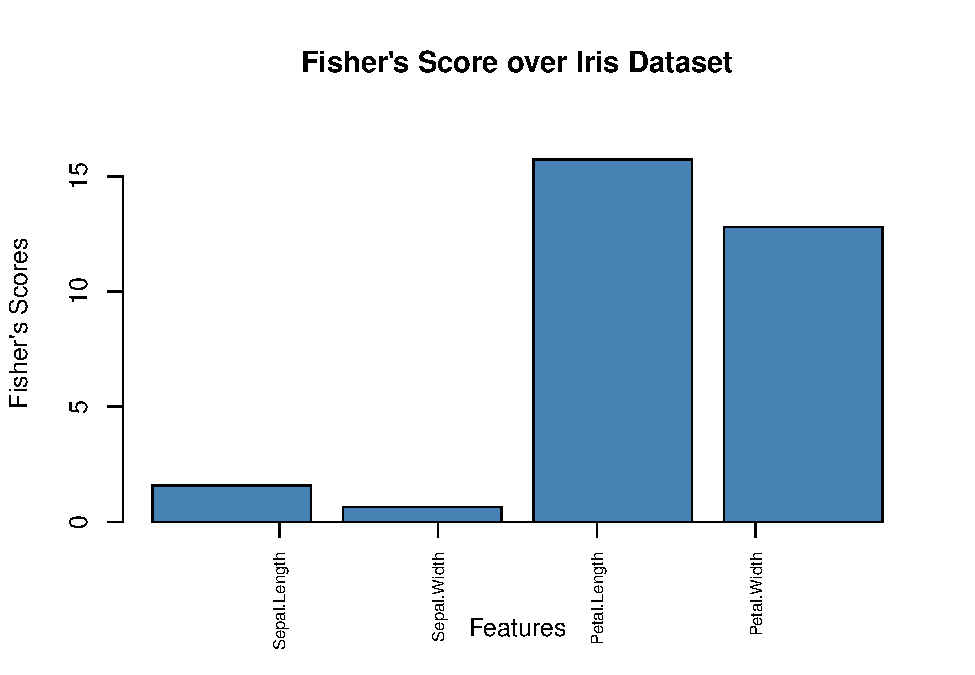
\includegraphics{figure/unnamed-chunk-4-1.pdf} you can see, from the
above bar Graph, Top features are Petal length, and petal width.

\hypertarget{sec:classification.}{%
\section{Classification.}\label{sec:classification.}}

A Decision Tree algorithm is one of the most popular machine learning
algorithms. It uses a tree like structure and their possible
combinations to solve a particular problem. It belongs to the class of
supervised learning algorithms where it can be used for both
classification and regression purposes.

A decision tree is a structure that includes a root node, branches, and
leaf nodes. Each internal node denotes a test on an attribute, each
branch denotes the outcome of a test, and each leaf node holds a class
label. The topmost node in the tree is the root node.

\hypertarget{sec:decision-tree}{%
\subsection{Decision Tree:}\label{sec:decision-tree}}

\begin{Shaded}
\begin{Highlighting}[]
\FunctionTok{library}\NormalTok{(here)}
\end{Highlighting}
\end{Shaded}

\begin{verbatim}
## here() starts at /home/rajeshkalakoti/Documents/data_mining_with_R
\end{verbatim}

\begin{Shaded}
\begin{Highlighting}[]
\FunctionTok{source}\NormalTok{(}\FunctionTok{here}\NormalTok{(}\StringTok{"RMarkDown/week5"}\NormalTok{,}
            \StringTok{"decision\_tree.R"}\NormalTok{))}
\end{Highlighting}
\end{Shaded}

\begin{verbatim}
## 
## Attaching package: 'dplyr'
\end{verbatim}

\begin{verbatim}
## The following objects are masked from 'package:stats':
## 
##     filter, lag
\end{verbatim}

\begin{verbatim}
## The following objects are masked from 'package:base':
## 
##     intersect, setdiff, setequal, union
\end{verbatim}

\hypertarget{sec:splitting-data}{%
\subsubsection{Splitting Data}\label{sec:splitting-data}}

\begin{Shaded}
\begin{Highlighting}[]
\FunctionTok{data}\NormalTok{(iris)}
\NormalTok{iris\_data }\OtherTok{\textless{}{-}}\NormalTok{ iris[iris}\SpecialCharTok{$}\NormalTok{Species }\SpecialCharTok{!=} \StringTok{\textquotesingle{}setosa\textquotesingle{}}\NormalTok{,]}
\NormalTok{input\_data }\OtherTok{\textless{}{-}}\NormalTok{ iris\_data}

\NormalTok{train\_index }\OtherTok{\textless{}{-}} \FunctionTok{sample}\NormalTok{(}\FunctionTok{row.names}\NormalTok{(input\_data),}
                      \FunctionTok{nrow}\NormalTok{(input\_data) }\SpecialCharTok{*} \FloatTok{0.66}\NormalTok{)}
\NormalTok{test\_index }\OtherTok{\textless{}{-}} \FunctionTok{row.names}\NormalTok{(input\_data)[}\SpecialCharTok{!}\FunctionTok{row.names}\NormalTok{(}
\NormalTok{  input\_data) }\SpecialCharTok{\%in\%}\NormalTok{ train\_index]}

\NormalTok{input\_train }\OtherTok{\textless{}{-}}\NormalTok{ input\_data[train\_index,]}
\NormalTok{input\_test }\OtherTok{\textless{}{-}}\NormalTok{ input\_data[test\_index,]}
\end{Highlighting}
\end{Shaded}

\hypertarget{sec:fitting-decision-tree}{%
\subsubsection{Fitting Decision Tree}\label{sec:fitting-decision-tree}}

\begin{Shaded}
\begin{Highlighting}[]
\NormalTok{tree\_rules }\OtherTok{\textless{}{-}} \FunctionTok{fit.decision.tree}\NormalTok{(}
\NormalTok{  input\_train,}\AttributeTok{min\_observations =} \DecValTok{3}\NormalTok{)}
\NormalTok{tree\_rules}
\NormalTok{input\_train}\SpecialCharTok{$}\NormalTok{regions }\OtherTok{\textless{}{-}} \FunctionTok{apply}\NormalTok{(input\_train,}\DecValTok{1}\NormalTok{,}
\NormalTok{                             identify\_region,}
\NormalTok{                             tree\_rules)}
\NormalTok{err\_rate\_vals }\OtherTok{\textless{}{-}} \FunctionTok{error\_rate}\NormalTok{(input\_train,}
                            \StringTok{"Species"}\NormalTok{,}
                            \StringTok{"regions"}\NormalTok{)}
\FunctionTok{print}\NormalTok{(}\StringTok{"Training Error Rate"}\NormalTok{)}
\FunctionTok{print}\NormalTok{(err\_rate\_vals[[}\DecValTok{1}\NormalTok{]])}
\NormalTok{class\_prob }\OtherTok{\textless{}{-}}\NormalTok{ err\_rate\_vals[[}\DecValTok{2}\NormalTok{]]}
\end{Highlighting}
\end{Shaded}

\hypertarget{sec:prediction-over-the-test-data}{%
\subsubsection{Prediction over the Test
data}\label{sec:prediction-over-the-test-data}}

\begin{Shaded}
\begin{Highlighting}[]
\NormalTok{test\_with\_preds }\OtherTok{\textless{}{-}} \FunctionTok{predict\_test}\NormalTok{(input\_test,}
\NormalTok{                                tree\_rules,}
\NormalTok{                                class\_prob)}

\NormalTok{preds\_table }\OtherTok{\textless{}{-}}\NormalTok{ test\_with\_preds[}\FunctionTok{c}\NormalTok{(}\StringTok{"Species"}\NormalTok{,}
                              \StringTok{"predict\_class"}\NormalTok{)] }
\end{Highlighting}
\end{Shaded}

\hypertarget{sec:classification-evaluation.}{%
\subsubsection{Classification
Evaluation.}\label{sec:classification-evaluation.}}

In the context of binary classification (where there are two classes,
typically denoted as positive and negative), true positives (TP), false
positives (FP), true negatives (TN), and false negatives (FN) are used
to evaluate the performance of a classification model. These values help
in understanding how well the model is performing in terms of correctly
and incorrectly predicting the classes.

Here's how you calculate these values based on model predictions and
actual outcomes:

\textbf{True Positives (TP):} These are the cases where the model
correctly predicts the positive class.

\textbf{False Positives (FP):} These are the cases where the model
incorrectly predicts the positive class when it should have been
negative.

\textbf{True Negatives (TN):} These are the cases where the model
correctly predicts the negative class.

\textbf{False Negatives (FN):} These are the cases where the model
incorrectly predicts the negative class when it should have been
positive.

Let's assume you have a set of predictions and the corresponding actual
outcomes:

Predicted: {[}1, 0, 1, 1, 0, 1{]} Actual: {[}1, 1, 1, 0, 0, 1{]}

To calculate TP, FP, TN, and FN based on these predictions:

\begin{itemize}
\item
  \textbf{True Positives (TP):} Count the number of cases where both
  predicted and actual values are 1. In this case, there are 3 instances
  (indices 1, 3, and 5).
\item
  \textbf{False Positives (FP):} Count the number of cases where the
  predicted value is 1, but the actual value is 0. In this case, there
  is 1 instance (index 0).
\item
  \textbf{True Negatives (TN):} Count the number of cases where both
  predicted and actual values are 0. In this case, there are 2 instances
  (indices 4 and 5).
\item
  \textbf{False Negatives (FN):} Count the number of cases where the
  predicted value is 0, but the actual value is 1. In this case, there
  is 1 instance (index 2).
\end{itemize}

So, based on these calculations:

\begin{itemize}
\tightlist
\item
  \textbf{TP = 3}
\item
  \textbf{FP = 1}
\item
  \textbf{TN = 2}
\item
  \textbf{FN = 1}
\end{itemize}

The metrics mentioned below (Precision, Recall, True Negative Rate
(Specificity), and Accuracy) are all calculated based on the values of
True Positives (TP), True Negatives (TN), False Positives (FP), and
False Negatives (FN). These metrics provide different perspectives on
the performance of a classification model and are essential in
evaluating the model's effectiveness using these fundamental elements of
classification results.

\begin{itemize}
\item
  \textbf{Precision:} Precision is calculated as:

  \[
  \text{Precision} = \frac{\text{TP}}{\text{TP + FP}}
  \]
\item
  \textbf{Recall:} Recall is calculated as:

  \[
  \text{Recall} = \frac{\text{TP}}{\text{TP + FN}}
  \]
\item
  \textbf{True Negative Rate (Specificity):} True Negative Rate, also
  known as Specificity, is calculated as:

  \[
  \text{TNR} = \frac{\text{TN}}{\text{TN + FP}}
  \]
\item
  \textbf{Accuracy:} Accuracy is calculated as:

  \[
  \text{Accuracy} = \frac{\text{TP + TN}}{\text{TP + TN + FP + FN}}
  \]
\item
  \textbf{Predicted Positive Condition Rate:} Predicted Positive
  Condition Rate is calculated as:

  \[
  \text{Predicted Positive Condition Rate} = \frac{\text{TP + FP}}{\text{TP + TN + FP + FN}}
  \]
\end{itemize}

\begin{Shaded}
\begin{Highlighting}[]
\FunctionTok{library}\NormalTok{(here)}
\FunctionTok{source}\NormalTok{(}\FunctionTok{here}\NormalTok{(}\StringTok{"RMarkDown/week5"}\NormalTok{,}
            \StringTok{"confusion\_matrix\_.R"}\NormalTok{))}
\NormalTok{results }\OtherTok{=} \FunctionTok{ConfusionMatrix}\NormalTok{(preds\_table}\SpecialCharTok{$}\NormalTok{Species,}
\NormalTok{                preds\_table}\SpecialCharTok{$}\NormalTok{predict\_class)}

\CommentTok{\# Calculate Accuracy}
\NormalTok{accuracy }\OtherTok{\textless{}{-}}\NormalTok{ results}\SpecialCharTok{$}\NormalTok{Accuracy}
\FunctionTok{print}\NormalTok{(}\FunctionTok{paste}\NormalTok{(}\StringTok{"Accuracy:"}\NormalTok{, accuracy))}
\end{Highlighting}
\end{Shaded}

\begin{verbatim}
## [1] "Accuracy: 0.824"
\end{verbatim}

\begin{Shaded}
\begin{Highlighting}[]
\CommentTok{\# Calculate Precision}
\NormalTok{precision }\OtherTok{\textless{}{-}}\NormalTok{ results}\SpecialCharTok{$}\NormalTok{Precision}
\FunctionTok{print}\NormalTok{(}\FunctionTok{paste}\NormalTok{(}\StringTok{"Precision:"}\NormalTok{, precision))}
\end{Highlighting}
\end{Shaded}

\begin{verbatim}
## [1] "Precision: 0.833"
\end{verbatim}

\begin{Shaded}
\begin{Highlighting}[]
\CommentTok{\# Calculate F1{-}Score}
\NormalTok{f1\_score }\OtherTok{\textless{}{-}}\NormalTok{ results}\SpecialCharTok{$}\NormalTok{F1\_Score}
\FunctionTok{print}\NormalTok{(}\FunctionTok{paste}\NormalTok{(}\StringTok{"F1{-}Score:"}\NormalTok{, f1\_score))}
\end{Highlighting}
\end{Shaded}

\begin{verbatim}
## [1] "F1-Score: 0.833"
\end{verbatim}

\begin{Shaded}
\begin{Highlighting}[]
\CommentTok{\# Calculate Sensitivity }
\CommentTok{\#(True Positive Rate or Recall)}
\NormalTok{sensitivity }\OtherTok{\textless{}{-}}\NormalTok{ results}\SpecialCharTok{$}\NormalTok{Sensitivity}
\FunctionTok{print}\NormalTok{(}\FunctionTok{paste}\NormalTok{(}\StringTok{"Sensitivity(Recall):"}\NormalTok{,}
\NormalTok{            sensitivity))}
\end{Highlighting}
\end{Shaded}

\begin{verbatim}
## [1] "Sensitivity(Recall): 0.833"
\end{verbatim}

\begin{Shaded}
\begin{Highlighting}[]
\CommentTok{\# Calculate AUC (Area Under the Curve)}
\NormalTok{auc }\OtherTok{\textless{}{-}}\NormalTok{ results}\SpecialCharTok{$}\NormalTok{AUC}
\FunctionTok{print}\NormalTok{(}\FunctionTok{paste}\NormalTok{(}\StringTok{"AUC (Area Under the Curve):"}
\NormalTok{            , auc))}
\end{Highlighting}
\end{Shaded}

\begin{verbatim}
## [1] "AUC (Area Under the Curve): 0.823"
\end{verbatim}

\hypertarget{sec:k-nearest-neighbour-k-nn-classification}{%
\subsection{k-nearest neighbour (k-NN)
classification}\label{sec:k-nearest-neighbour-k-nn-classification}}

Let \(N\) be a labeled set of points belonging to \(c\) different
classes such that
\begin{equation}\protect\hypertarget{eq:knn}{}{ \sum_{i=1}^{c} N_i = N }\end{equation}
During the classification of a given point \(x\), the algorithm
identifies the \(k\) nearest points to \(x\) and assigns \(x\) the
majority label among its \(k\) nearest neighbors. K-NN relies on the
concept of proximity, and for this, it employs a distance function to
calculate the distances between points.

\begin{Shaded}
\begin{Highlighting}[]
\FunctionTok{library}\NormalTok{(here)}
\FunctionTok{source}\NormalTok{(}\FunctionTok{here}\NormalTok{(}\StringTok{"RMarkDown/week5"}\NormalTok{,}\StringTok{"knn\_classification.R"}\NormalTok{))}
\end{Highlighting}
\end{Shaded}

\begin{verbatim}
## -- Attaching core tidyverse packages ------------------------ tidyverse 2.0.0 --
## v forcats   1.0.0     v readr     2.1.4
## v ggplot2   3.4.3     v stringr   1.5.0
## v lubridate 1.9.2     v tibble    3.2.1
## v purrr     1.0.1     v tidyr     1.3.0
## -- Conflicts ------------------------------------------ tidyverse_conflicts() --
## x dplyr::filter() masks stats::filter()
## x dplyr::lag()    masks stats::lag()
## i Use the conflicted package (<http://conflicted.r-lib.org/>) to force all conflicts to become errors
## 
## Attaching package: 'reshape'
## 
## 
## The following object is masked from 'package:lubridate':
## 
##     stamp
## 
## 
## The following objects are masked from 'package:tidyr':
## 
##     expand, smiths
## 
## 
## The following object is masked from 'package:dplyr':
## 
##     rename
\end{verbatim}

\begin{Shaded}
\begin{Highlighting}[]
\FunctionTok{data}\NormalTok{(iris)}

\NormalTok{labels }\OtherTok{\textless{}{-}}\NormalTok{ iris}\SpecialCharTok{$}\NormalTok{Species}
\NormalTok{data }\OtherTok{\textless{}{-}}\NormalTok{ iris[, }\SpecialCharTok{{-}}\DecValTok{5}\NormalTok{]}
\FunctionTok{suppressMessages}\NormalTok{(}\FunctionTok{eval\_knn}\NormalTok{(}
\NormalTok{  data, labels,}
  \AttributeTok{k\_neighbors=}\FunctionTok{seq}\NormalTok{(}\DecValTok{5}\NormalTok{, }\DecValTok{19}\NormalTok{, }\AttributeTok{by=}\DecValTok{2}\NormalTok{),}
  \AttributeTok{metrics =} \FunctionTok{c}\NormalTok{(}\StringTok{"euclidean"}\NormalTok{, }\StringTok{"manhattan"}\NormalTok{)))}
\end{Highlighting}
\end{Shaded}

\begin{verbatim}
## [1] "Going for method euclidean"
## [1] "Going for method manhattan"
\end{verbatim}

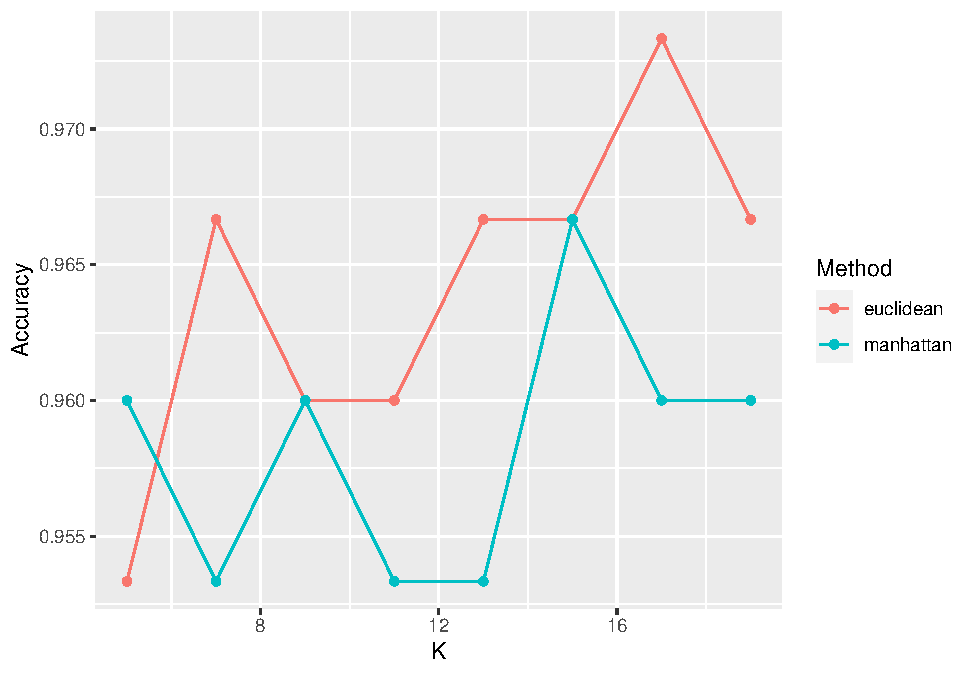
\includegraphics{figure/unnamed-chunk-11-1.pdf}

\begin{verbatim}
##       Method  K  Accuracy
## 1  euclidean  5 0.9533333
## 2  euclidean  7 0.9666667
## 3  euclidean  9 0.9600000
## 4  euclidean 11 0.9600000
## 5  euclidean 13 0.9666667
## 6  euclidean 15 0.9666667
## 7  euclidean 17 0.9733333
## 8  euclidean 19 0.9666667
## 9  manhattan  5 0.9600000
## 10 manhattan  7 0.9533333
## 11 manhattan  9 0.9600000
## 12 manhattan 11 0.9533333
## 13 manhattan 13 0.9533333
## 14 manhattan 15 0.9666667
## 15 manhattan 17 0.9600000
## 16 manhattan 19 0.9600000
\end{verbatim}

\hypertarget{sec:naive-bayes}{%
\subsection{Naive Bayes}\label{sec:naive-bayes}}

It is based on Bayes' theorem with an assumption of independence between
features. The ``naive'' assumption here implies that the presence of a
particular feature in a class is independent of the presence of other
features. This assumption simplifies the calculation process.

In Naive Bayes classification, the probability of a class \(C_k\) given
the features \(x\) is calculated using Bayes' theorem as follows:

\[ P(C_k | x) = \frac{{P(x | C_k) \times P(C_k)}}{{P(x)}} \]

Where: - \(P(C_k | x)\) is the posterior probability of class \(C_k\)
given features \(x\). - \(P(x | C_k)\) is the likelihood, representing
the probability of observing the features \(x\) given class \(C_k\). -
\(P(C_k)\) is the prior probability of class \(C_k\). - \(P(x)\) is the
probability of observing the features \(x\).

This equation is fundamental to the Naive Bayes classification
algorithm.

\[ y^* = \text{argmax}_{y \in \{0,1\}} \, p(y | x, \theta) \]

here i have used the package ``e1071'', you can install it.

\begin{Shaded}
\begin{Highlighting}[]
\FunctionTok{library}\NormalTok{(e1071)}
\CommentTok{\# Set a seed for reproducibility}
\FunctionTok{set.seed}\NormalTok{(}\DecValTok{123}\NormalTok{)}


\NormalTok{split\_index }\OtherTok{\textless{}{-}} \FunctionTok{sample}\NormalTok{(}\DecValTok{1}\SpecialCharTok{:}\FunctionTok{nrow}\NormalTok{(iris),}
                      \FloatTok{0.7} \SpecialCharTok{*} \FunctionTok{nrow}\NormalTok{(iris))}
\NormalTok{train\_data }\OtherTok{\textless{}{-}}\NormalTok{ iris[split\_index, ]}
\NormalTok{test\_data }\OtherTok{\textless{}{-}}\NormalTok{ iris[}\SpecialCharTok{{-}}\NormalTok{split\_index, ]}

\NormalTok{naive\_bayes\_model }\OtherTok{\textless{}{-}} \FunctionTok{naiveBayes}\NormalTok{(}
\NormalTok{Species }\SpecialCharTok{\textasciitilde{}}\NormalTok{ Sepal.Length }\SpecialCharTok{+}\NormalTok{ Sepal.Width,}
\AttributeTok{data =}\NormalTok{ train\_data)}
\CommentTok{\# Make predictions on the test data}
\NormalTok{predictions }\OtherTok{\textless{}{-}} \FunctionTok{predict}\NormalTok{(naive\_bayes\_model,}
\AttributeTok{newdata =}\NormalTok{ test\_data)}
\NormalTok{actual\_labels }\OtherTok{=}\NormalTok{ test\_data}\SpecialCharTok{$}\NormalTok{Species}
\end{Highlighting}
\end{Shaded}

\hypertarget{sec:classification-evaluation}{%
\subsubsection{Classification
Evaluation}\label{sec:classification-evaluation}}

Naive Bayes Classification Results.

\begin{Shaded}
\begin{Highlighting}[]
\FunctionTok{library}\NormalTok{(here)}
\FunctionTok{source}\NormalTok{(}\FunctionTok{here}\NormalTok{(}\StringTok{"RMarkDown/week5"}\NormalTok{,}
            \StringTok{"confusion\_matrix\_.R"}\NormalTok{))}
\NormalTok{results }\OtherTok{=} \FunctionTok{ConfusionMatrix}\NormalTok{(}
\FunctionTok{as.character}\NormalTok{(predictions),}
\NormalTok{actual\_labels)}
\end{Highlighting}
\end{Shaded}

\begin{Shaded}
\begin{Highlighting}[]
 \FunctionTok{print}\NormalTok{(}\FunctionTok{xtable}\NormalTok{(}
\NormalTok{   results,}
   \AttributeTok{caption=}\StringTok{\textquotesingle{}confusion matrix results\textquotesingle{}}\NormalTok{,}
   \AttributeTok{label=}\StringTok{\textquotesingle{}tbl:results.xtable\textquotesingle{}}\NormalTok{,}
   \AttributeTok{align=}\FunctionTok{c}\NormalTok{(}\FunctionTok{rep}\NormalTok{(}\StringTok{\textquotesingle{}r\textquotesingle{}}\NormalTok{, }\DecValTok{6}\NormalTok{), }\StringTok{\textquotesingle{}l\textquotesingle{}}\NormalTok{)))}
\end{Highlighting}
\end{Shaded}

\begin{table}[!t]
\centering
\caption{confusion matrix results} 
\label{tbl:results.xtable}
\begin{tabular}{rrrrrl}
  \hline
Accuracy & Precision & Sensitivity & F1\_Score & Specificity & AUC\_average \\ 
  \hline
0.98 & 1.00 & 0.93 & 0.97 & 1.00 & 0.90 \\ 
  0.80 & 0.67 & 0.80 & 0.73 & 0.80 & 0.90 \\ 
  0.82 & 0.77 & 0.67 & 0.71 & 0.90 & 0.90 \\ 
   \hline
\end{tabular}
\end{table}

\bibliography{IEEEabrv,./library}

\end{document}
